\documentclass{homework}
\usepackage{enumitem}

\newcommand{\hwclass}{Math 6108}
\newcommand{\hwname}{Jacob Hauck}
\newcommand{\hwtype}{Homework}

\newcommand{\R}{\textbf{R}}
\newcommand{\dee}{\;\text{d}}
\newcommand{\eps}{\varepsilon}
\newcommand{\pl}[2]{\frac{\partial #1}{\partial #2}}
\newcommand{\dl}[2]{\frac{\text{d} #1}{\text{d} #2}}
\newcommand{\sgn}{\text{sgn}}
\newcommand{\bigoh}{\mathcal{O}}

\usepackage{tikz}
\usepackage{pgfplots}
\pgfplotsset{compat=1.18}

\newcommand{\hwnum}{3}
\renewcommand{\questiontype}{Problem}

\begin{document}
	\maketitle
	
	\question
	\begin{alphaparts}
		\questionpart To find the best approximation $p \in P^3[-1,1]$ of $f(t) = \sin(t)$ on $[-1,1]$, we simply use the definition. If $p$ is the best approximation, then
		\begin{equation}
			E(q) = \lVert q - f \rVert_{L^2}
		\end{equation}
		must be minimal with respect to $q \in P^3[-1,1]$ if $q = p$. Since every element $q \in P^3[-1,1]$ satisfies $q(t) = q_0 + q_1 t + q_2 t^2 + q_3t^3$ for some $\{q_i\}_{i=0}^3 \in \R^4$, and $E$ is minimal precisely when $E^2$ is minimal, it follows that the representation $\{p_i\} \in \R^4$ of $p$ is the minimizer of
		\begin{equation}
			\label{eq:integral_error}
			F(\{q_i\}) = E^2(q) = \lVert q- f\rVert_{L^2}^2 = \int_{-1}^1(q_0 + q_1t + q_2t^2 + q_3 t^3 - \sin(t))^2\dee t
		\end{equation}
		with respect to $\{q_i\} \in \R^4$. Since $F$ is clearly continuously differentiable, the Extreme Value Theorem implies that its gradient is 0 when $\{q_i\} = \{p_i\}$ because $\{p_i\}$ is a minimizer of $F$. Therefore,
		\begin{equation}
			\pl{F}{q_i}(\{p_i\}) = \int_{-1}^12(p_0+p_1t + p_2t^2 + p_3t^3 - \sin(t))t^i\dee t = 0
		\end{equation}
		for $i \in \{0,1,2,3\}$. Then
		\begin{align}
			0 &= \int_{-1}^1(p_0t^i + p_1t^{i+1} + p_2t^{i+2} + p_3t^{i+3} - t^i\sin(t))\dee t \\
			\label{eq:gradient}
			&= \left[\frac{p_0}{i+1}t^{i+1} + \frac{p_1}{i+2}t^{i+2} + \frac{p_2}{i+3}t^{i+3} + \frac{p_3}{i+4}t^{i+4}\right]_{-1}^1 - \int_{-1}^1 t^i \sin(t)\dee t.
		\end{align}
		Note that $t^i\sin(t)$ is odd if $i$ is even, which makes $\int_{-1}^1t^{i}\sin(t)\dee t = 0$. If $i$ is odd, then $i \in \{1,3\}$, and
		\begin{equation}
			\int_{-1}^1 t\sin(t)\dee t = \big[-t\cos(t) + \sin(t)\big]_{-1}^1 = 2\sin(1)-2\cos(1)
		\end{equation}
		and
		\begin{equation}
			\int_{-1}^1 t^3\sin(t)\dee t = \big[-t^3\cos(t) +3t^2\sin(t) + 6t\cos(t) - 6\sin(t)\big]_{-1}^1 = 10\cos(1) -6\sin(1)
		\end{equation}
		Evaluating (\ref{eq:integral_error}) for $i \in \{0,1,2,3\}$, we obtain a system of four equations
		\begin{alignat}{2}
			(i=0)&& \qquad 0 &= 2p_0+ \frac{2}{3}p_2, \\
			(i=1)&& \qquad 2\sin(1)-2\cos(1) &= \frac{2}{3}p_1 + \frac{2}{5}p_3, \\
			(i=2)&& \qquad 0 &= \frac{2}{3}p_0 + \frac{2}{5}p_2, \\
			(i=3)&& \qquad 10\cos(1) -6\sin(1) &= \frac{2}{5}p_1 + \frac{2}{7}p_3.
		\end{alignat}
		Using substitution on the first and third equations, we see that $p_0 = -\frac{1}{3}p_2$, so that $\frac{8}{45}p_2 = 0$. Thus, $p_0 = p_2 = 0$ (as expected, since $\sin$ is odd). Solving the second pair of equations is less fun; if $x = (p_1, p_3)^T$, then $x$ solves the equation
		\begin{equation}
			\left[\begin{matrix}
				\frac{2}{3} & \frac{2}{5} \\[0.5em]
				\frac{2}{5} & \frac{2}{7}
			\end{matrix}\right] x = \left[\begin{matrix}
				-2 \\
				10
			\end{matrix}\right]\cos(1) + \left[\begin{matrix}
			2 \\
			-6
		\end{matrix}\right]\sin(1).
		\end{equation}
		Using the formula for $2\times 2$ inverse matrices gives
		\begin{align}
			x &= \frac{1}{\frac{4}{21} - \frac{4}{25}}\left[\begin{matrix}
				\frac{2}{7} & -\frac{2}{5} \\[0.5em]
				-\frac{2}{5} & \frac{2}{3}
			\end{matrix}\right]\left(\left[\begin{matrix}
				-2 \\
				10
			\end{matrix}\right]\cos(1) + \left[\begin{matrix}
				2 \\
				-6
			\end{matrix}\right]\sin(1)\right) \\[0.5em]
			&= \frac{525}{16}\left(\left[\begin{matrix}
				-\frac{32}{7} \\[0.5em]
				\frac{112}{15}
			\end{matrix}\right]\cos(1) + \left[\begin{matrix}
				\frac{104}{35} \\[0.5em]
				-\frac{24}{5}
			\end{matrix}\right]\sin(1)\right)\\[0.5em]
			&= \left[\begin{matrix}
				-150\cos(1) + \frac{195}{2}\sin(1) \\[0.5em]
				245\cos(1) - \frac{315}{2}\sin(1)
			\end{matrix}\right].
		\end{align}
		That is, $p_1 = -150\cos(1) + \frac{195}{2}\sin(1)$ and $p_3 = 245\cos(1) - \frac{315}{2}\sin(1)$, and the best approximation $p \in P^3[-1,1]$ of $f$ on $[-1,1]$ in $L^2$ norm is
		\begin{align}
			p(t) &= \left(-150\cos(1) + \frac{195}{2}\sin(1)\right)t + \left(245\cos(1) - \frac{315}{2}\sin(1)\right)t^3 \\
			&\approx 0.998075139 t - 0.157615170 t^3
		\end{align}
		\begin{figure}
		\centering
		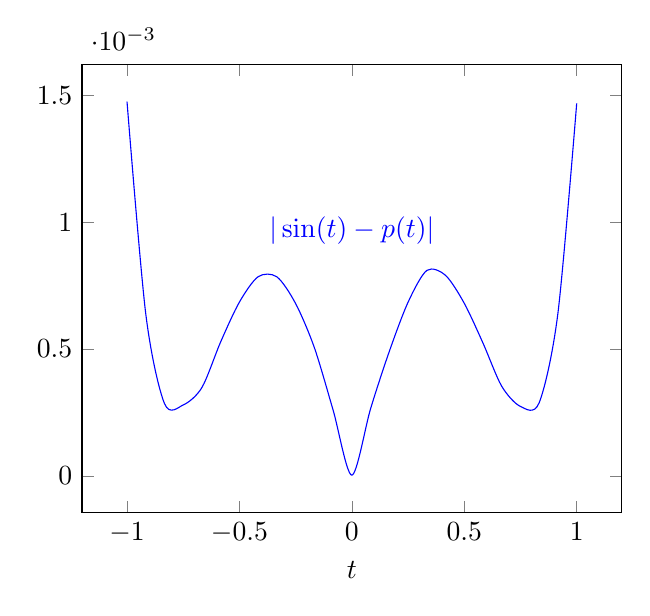
\begin{tikzpicture}
			\begin{axis}[domain=-1:1, xlabel={$t$}, smooth]
				\addplot[mark=none, blue] {abs(sin(deg(x)) - ((-150*cos(deg(1)) + 195/2*sin(deg(1))) * x + (245*cos(deg(1)) - 315/2*sin(deg(1))) * x * x * x))} node [midway, above=8em] {$|\sin(t) - p(t)|$};
			\end{axis}
		\end{tikzpicture}
		\caption{Absolute error between $p$ and $\sin$ on $[-1,1]$. Evidently, the approximation is pretty good.}
		\label{fig:best_l2_error}
		\end{figure}
		Figure \ref{fig:best_l2_error} provides a visualization of the approximation error.
		
		\questionpart The degree 3 Taylor approximation polynomial $p(t)$ for $f(t) = \sin(t)$ centered at $t=0$ is defined to be
		\begin{equation}
			p(t) = \sum_{n=0}^3 \frac{f^{(n)}(0)}{n!}x^n = x - \frac{x^3}{6}
		\end{equation}
		because $f(0) = 0$, $f'(0) = \cos(0) = 1$, $f''(0) = -\sin(0) = 0$, and $f'''(0) = -\cos(0) = -1$. Note how the coefficients are fairly close to those found in the previous part (the best $L^2$ approximation). Figure \ref{fig:taylor_error} gives a visualization of the absolute error between $p$ and $f = \sin$. Note how the error is smaller near $t=0$ but larger away from $t=0$ than the best $L^2$ approximation error.
		
		\begin{figure}
			\centering
			\begin{tikzpicture}
				\begin{axis}[domain=-1:1, xlabel={$t$}, smooth]
					\addplot[mark=none, blue] {abs(sin(deg(x)) - x + x*x*x/6)} node [midway, above=8em] {$|\sin(t) - p(t)|$};
				\end{axis}
			\end{tikzpicture}
			\caption{Absolute error between $p$ and $\sin$ on $[-1,1]$. This approximation is also pretty good.}
			\label{fig:taylor_error}
		\end{figure}
		
		\questionpart The degree 3 Lagrange polynomial approximation of $f(t) = \sin(t)$ that interpolates at the points $T = \left\{-1,-\frac{1}{3},\frac{1}{3}, 1\right\}$ is defined to be the degree 3 polynomial $p$ such that $p(t) = f(t)$ for all $t \in T$. There are numbers $\{p_i\}_{i=0}^3 \in \R^4$ such that $p(t) = p_0 + p_1t + p_2t^2 + p_3t^3$; the definition of $p$ therefore requires that the following equations be true
		\begin{align}
			\sin(-1) &= p_0 - p_1 + p_2 - p_3, \\
			\sin\left(-\frac{1}{3}\right) &= p_0 - \frac{1}{3}p_1 + \frac{1}{9}p_2 - \frac{1}{27}p_3, \\
			\sin\left(\frac{1}{3}\right) &= p_0 + \frac{1}{3}p_1 + \frac{1}{9}p_2 + \frac{1}{27}p_3, \\
			\sin(1) &= p_0 + p_1 + p_2 + p_3.
		\end{align}
		Adding the first and last equations, we get $2p_0 + 2p_2 = 0$, so $p_0 = -p_2$. Adding the middle two equations, we get $2p_0 + \frac{2}{9}p_2 =0$, which implies that $\frac{17}{9}p_0 = 0$, so $p_0 = 0 = p_2$ (as expected from the oddness of $\sin$ and odd symmetry of $T$). 
		
		Subtracting the first equation from the last, we get $p_1 + p_3 = \sin(1)$. Subracting the third equation from the second, we get $\frac{1}{3}p_1 + \frac{1}{27}p_3 = \sin\left(\frac{1}{3}\right)$, or $9p_1 + p_3 = 27\sin\left(\frac{1}{3}\right)$. Therefore, $\sin(1) - p_1 = 27\sin\left(\frac{1}{3}\right) - 9p_1$, which implies that $p_1 = \frac{1}{8}\left(27\sin\left(\frac{1}{3}\right) - \sin(1)\right)$, and $p_3 = \sin(1) - p_1 = \frac{1}{8}\left(9\sin(1) - 27\sin\left(\frac{1}{3}\right)\right)$. Thus,
		\begin{align}
			p(t) &=  \frac{1}{8}\left(27\sin\left(\frac{1}{3}\right) - \sin(1)\right)t + \frac{1}{8}\left(9\sin(1) - 27\sin\left(\frac{1}{3}\right)\right)t^3\\
			&\approx 0.999098228 t - 0.157627243 t^3.
		\end{align}
		
		\begin{figure}
			\centering
			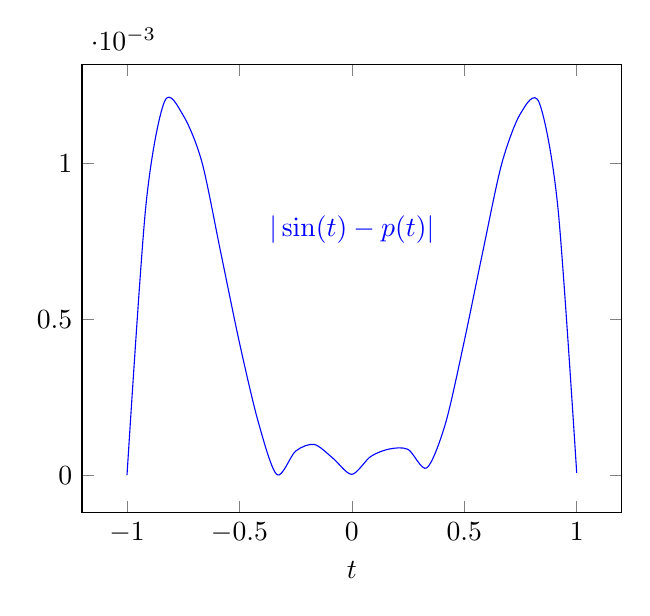
\begin{tikzpicture}
				\begin{axis}[domain=-1:1, xlabel={$t$}, smooth]
					\addplot[mark=none, blue] {abs(sin(deg(x)) - (1/8*(27*sin(deg(1/3)) - sin(deg(1))) * x + 1/8*(9*sin(deg(1)) - 27*sin(deg(1/3)))*x*x*x))} node [midway, above=8em] {$|\sin(t) - p(t)|$};
				\end{axis}
			\end{tikzpicture}
			\caption{Absolute error between $p$ and $\sin$ on $[-1,1]$. This approximation is also quite good.}
			\label{fig:lagrange_error}
		\end{figure}
		Figure \ref{fig:lagrange_error} shows a visulization of the error between $p$ and $f$. Note that the error is $0$ when $t \in T$, and also when $t= 0$ because of the oddness of both $p$ and $f$.
	\end{alphaparts}
	
	\question First, we find $w_1 = \frac{u_1}{\lVert u_1\rVert}$. Since
	\begin{equation}
		\lVert u_1\rVert^2 = \int_0^1 1^2 \dee x = 1,
	\end{equation}
	we get $\lVert u_1 \rVert = 1$, and $w_1 = 1$. By the Gram-Schmidt process, $v_2 = u_2 - (u_2, w_1) w_1$ is orthogonal to $w_1$. Since
	\begin{equation}
		(u_2, w_1) = \int_0^1 x\dee x = \frac{1}{2},
	\end{equation}
	it follows that $v_2 = x - \frac{1}{2}$ is orthogonal to $w_1$. Then $w_2 = \frac{v_2}{\lVert v_2\rVert}$ is orthogonal to $w_1$ and is a unit vector. Since
	\begin{equation}
		\lVert v_2\rVert^2 = \int_0^1 \left(x - \frac{1}{2}\right)^2\dee x = \left.\frac{1}{3}\left(x-\frac{1}{2}\right)^3\right\vert_0^1 = \frac{1}{12},
	\end{equation}
	it follows that $w_2 = \sqrt{12}x - \sqrt{3}$ is orthogonal to $w_1$ and is a unit vector. By the Gram-Schmidt process again, $v_3 = u_3 - (u_3,w_2)w_2 - (u_3,w_1)w_1$ is orthogonal to $w_1$ and to $w_2$. Since
	\begin{equation}
		(u_3, w_2) = \int_0^1 x^2\left(\sqrt{12}x - \sqrt{3}\right)\dee x = \frac{\sqrt{12}}{4}x^4 - \frac{\sqrt{3}}{3}x^3\Big\vert_0^1 = \frac{\sqrt{12}}{12},
	\end{equation}
	and
	\begin{equation}
		(u_3,w_1) = \int_0^1 x^2\dee x = \frac{1}{3},
	\end{equation}
	it follows that
	\begin{equation}
		v_3 = x^2 - x + \frac{1}{2} - \frac{1}{3} = x^2-x +\frac{1}{6}.
	\end{equation}
	Then $v_3$ is orthogonal to $w_1$ and $w_2$, and $w_3 = \frac{v_3}{\lVert v_3\rVert}$ is orthogonal to $w_1$ and $w_2$ and is a unit vector. Since
	\begin{equation}
		\lVert v_3\rVert^2 = \int_0^1 \left(x^2 - x +\frac{1}{6}\right)^2\dee x = \left[\frac{1}{5}x^5 - \frac{1}{2}x^4 + \frac{4}{9}x^3 - \frac{1}{6}x^2 +\frac{1}{36}x\right]_0^1 = \frac{1}{180}
	\end{equation}
	it follows that
	\begin{equation}
		w_3 = \sqrt{180}\left(x^2-x+\frac{1}{6}\right)
	\end{equation}
	is orthogonal to $w_1$ and $w_2$ and is a unit vector. Altogether then, the orthonormal basis for $P^2[0,1]$ obtained by the Gram-Schmidt process applied to $\{1,x,x^2\}$ is
	\begin{equation}
		B = \left\{1, \sqrt{12}x - \sqrt{3}, \sqrt{180}\left(x^2-x+\frac{1}{6}\right)\right\}
	\end{equation}
	The best approximation for $f(x) = \sqrt{x}$ in $P^2[0,1]$ with respect to the $L^2$ norm is therefore
	\begin{equation}
		p(x) = p_1w_1(x) + p_2w_2(x) + p_3w_3(x)
	\end{equation}
	where $p_i = (\sqrt{x}, w_i)$. Computing these inner products, we get
	\begin{align}
		p_1 &= (\sqrt{x}, w_1) = \int_0^1\sqrt{x}\dee x = \frac{2}{3}, \\
		p_2 &= (\sqrt{x}, w_2) = \int_0^1\sqrt{x}\left(\sqrt{12}x - \sqrt{3}\right)\dee x = \frac{2\sqrt{12}}{5} - \frac{2\sqrt{3}}{3} = \frac{\sqrt{12}}{15}, \\
		p_3 &= (\sqrt{x}, w_3) = \int_0^1 \sqrt{x}\cdot\sqrt{180}\left(x^2 - x + \frac{1}{6}\right)\dee x = \sqrt{180}\left(\frac{2}{7} - \frac{2}{5} + \frac{1}{9}\right) = -\frac{\sqrt{180}}{315}
	\end{align}
	Therefore, the best approximation is
	\begin{align}
		p(x) &= \frac{2}{3} + \frac{\sqrt{12}}{15}\left(\sqrt{12}x - \sqrt{3}\right) - \frac{180}{315}\left(x^2-x+\frac{1}{6}\right) \\
		&= \frac{2}{3} + \frac{4}{5}x - \frac{2}{5} - \frac{4}{7}x^2 + \frac{4}{7}x - \frac{2}{21} \\
		&= -\frac{4}{7}x^2 + \frac{48}{35}x +\frac{6}{35}\\
		&\approx -0.571428571 x^2 + 1.371428571x + 0.171428571
	\end{align}
	See figure \ref{fig:best_sqrt_error} for a visualization of the error.
	\begin{figure}	
		\centering
		\begin{tikzpicture}
			\begin{axis}[domain=0:1, xlabel={$x$}, samples=1000]
				\addplot[mark=none, blue] {abs(sqrt(x) + 4/7*x*x  - 48/35*x - 6/35)} node [midway, above=2em] {$|\sqrt{x} - p(x)|$};
			\end{axis}
		\end{tikzpicture}
		\caption{Absolute error between $p$ and $\sqrt{\cdot}$ on $[0,1]$}
		\label{fig:best_sqrt_error}
	\end{figure}
	
	\question Let $p$ be the quadratic polynomial satisfying $p(0) = f(0)$, $p(2) = f(2)$, and $p'(2) = f'(2)$. There exists $\{p_i\}_{i=0}^2 \in \R^3$ such that $p(x) = p_0 + p_1x + p_2x^2$. Since $p(0) = f(0)$, it follows that $p_0 = f(0)$. Since $p'(2) = p_1 + 4p_2 = f'(2)$, and $p(2) = f(0) + 2p_1+4p_2 = f(2)$, it follows that $f(2) - f'(2) = f(0) + p_1$, so $p_1 = f(2) - f'(2) - f(0)$, and $p_2 = \frac{1}{4}(f'(2) - p_1) = \frac{1}{4}(2f'(2)+f(0) - f(2))$. Therefore,
	\begin{equation}
		p(x) = p_0 + p_1x + p_2x^2 = f(0) + (f(2) - f'(2) - f(0))x + \frac{1}{4}(2f'(2) + f(0) - f(2))x^2
	\end{equation}
\end{document}